\chapter{Mininet-Wifi}

Por lo que he leído Mininet-Wifi no incorpora el estándar que usábamos para el estudio de las redes de área personal con tasa baja de transmisión de datos, 802.15.4 .
\section{Enlaces útiles}
\begin{itemize}
    \item Articulos sobre Mininet y Mininet-Wifi: \url{http://www.brianlinkletter.com/tag/mininet/}
    
\end{itemize}


\section{¿Qué es?}


Mininet-Wifi es un fork del proyecto Mininet con el que podías emular redes SDN, y se han extendido sus funcionalidades al ámbito de las redes wireless. Por lo que con el se pueden combinar ambas funcionalidades, las anteriores comunes a Mininet y las nuevas que incorpora Mininet-Wifi.

\section{¿Qué es el término RSSI?}

El indicador de fuerza de la señal recibida (RSSI por las siglas del inglés Received Signal Strength Indicator), es una escala de referencia \textbf{en relación a 1 mW} para medir el nivel de potencia de las señales recibidas por un dispositivo en las redes inalámbricas (típicamente WIFI o telefonía móvil).



% Please add the following required packages to your document preamble:
% \usepackage{booktabs}

\begin{table}[!htb]
\centering
\begin{tabular}{@{}ll@{}}
\toprule
RSSI & Descripción                                                                                                                                                        \\ \midrule
0    & Señal ideal                                                                                                                                                        \\
-40  & Señal idónea con tasas de transferencia estables.                                                                                                                  \\
-60  & \begin{tabular}[c]{@{}l@{}}Enlace bueno, ajustando la \\ transmisión (Tx) se puede lograr una conexión estable al 80\%\end{tabular}                                \\
-70  & \begin{tabular}[c]{@{}l@{}}Enlace medio-bajo, es una señal medianamente buena\\ aunque se pueden sufrir problemas con lluvia y viento.\end{tabular}                \\
-80  & \begin{tabular}[c]{@{}l@{}}Es la señal mínima aceptable para establecer la conexión.\\ Pueden ocurrir caídas que se traducen en corte de comunicación\end{tabular} \\ \bottomrule
\end{tabular}
\centering 
\end{table}

\newpage

\section{Instalación}

Instalar Mininet-Wifi me ha resultado muy sencillo. Se lleva a cabo vía un shellscript que te dan ya hecho al clonar el repositorio de Mininet-Wifi. Los pasos que he seguido en la instalación de Mininet-Wifi son:
\begin{itemize}
    \item Instalar una máquina virtual con Ubuntu 16.04
    \item Añadir git, sudo apt-get install git 
    \item Clonar el repositorio, git clone https://github.com/intrig-unicamp/mininet-wifi
    \item cd mininet-wifi
    \item Completar la instalación: sudo \textbf{util/install.sh -Wlnfv}
    \begin{itemize}
        \item -W: wireless dependencies
        \item -n: mininet-wifi dependencies
        \item -f: OpenFlow
        \item -v: OpenvSwitch
        \item -l: wmediumd
    \end{itemize}
    \item De forma adicional hemos instalado Wireshark para poder analizar los test realizados
\end{itemize}

\section{Test 1}
La red más sencilla es por defecto la red de un punto de acceso y dos estaciones wireless. El punto de acceso está conectado directamente al controlador, y las estaciones wireless serán los host. La idea de este test es comprobar que hay fluctuación de tráfico de control OpenFlow en el punto de acceso y además hay tráfico de usuario en la interfaz de wlan.

\begin{itemize}
    \item Lanzamos Wireshark para analizar tráfico: \textbf{wireshark \&}
    \item Lanzamos Mininet-Wifi con el siguiente comando, además por defecto cargará la topología por defecto(Valga la redundancia): \textbf{sudo mn -wifi}
    \item Lo siguiente, es activar la interfaz hwsim0. Pero, ¿Qué es la interfaz hwsim0? La interfaz hwsim0 es una interfaz software creada por Mininet-Wifi que copia todo el trafico wireless  dirigido a todas las interfaces wireless virtuales de la topología a emular. Según la documentación seguida es la forma más sencilla de monitorizar los mensajes wireless en Mininet-Wifi. Desde la Mininet-Wifi CLI: \textbf{sh ifconfig hwsim0 up} 
    \begin{itemize}
        \item El comando \textbf{sh} en la CLI de Mininet tiene la funcionalidad de ejecutar un comando fuera de la Interfaz de Mininet-Wifi.
    \end{itemize}
    
    \item Una vez levantada la interfaz podemos poner Wireshark a escuchar en la interfaz.
    
    \item Hacemos Ping desde la estación sta1, a la estación sta2: \textbf{sta1 ping sta2}
    
    \item Comprobamos que hay tráfico escuchando en la interfaz:
    
    
\end{itemize}
\newpage
\begin{figure}[!htb]
  \centering
    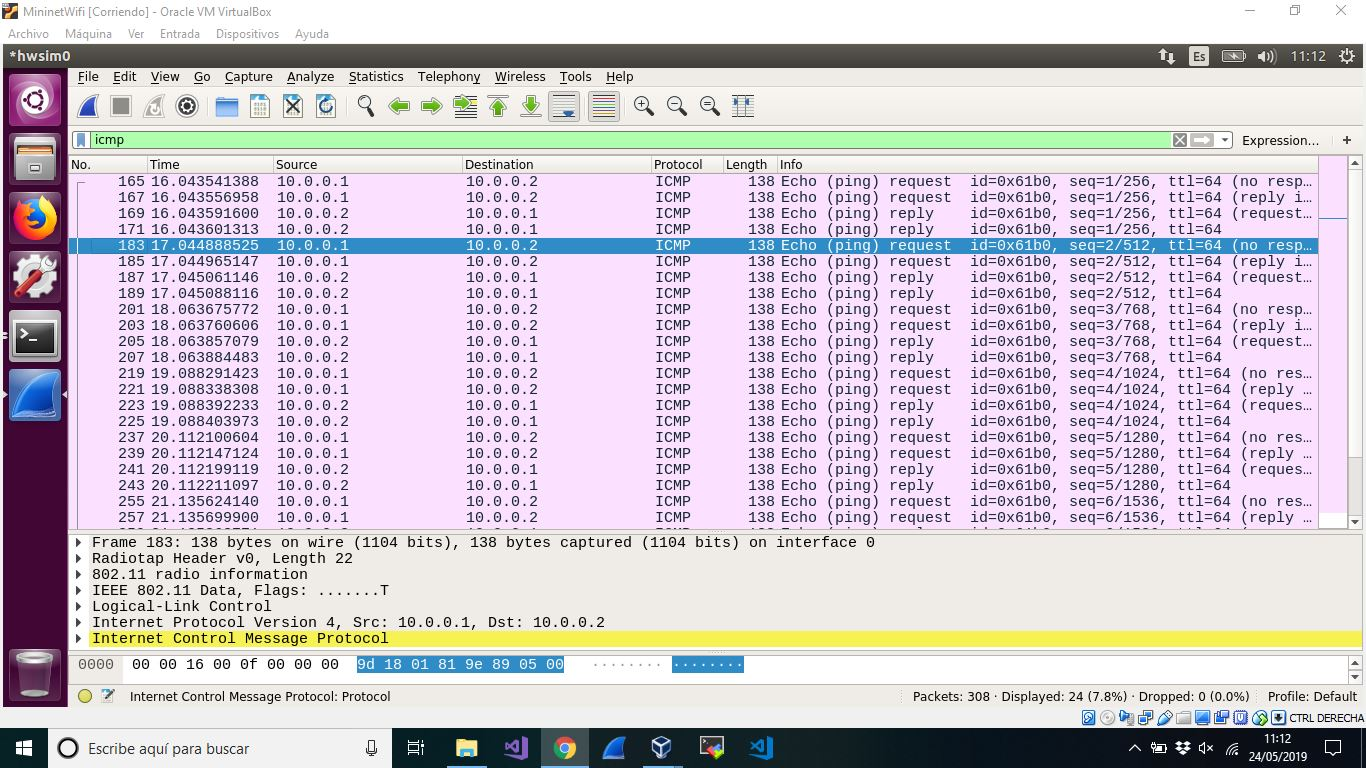
\includegraphics[width=\linewidth]{./img/5.JPG}
    \caption{Comprobación que hay trafico a través de la interfaz.}
  \label{fig:yo}
\end{figure}

Como podeos ver el punto de acceso tiene una interfaz asociada llamada ap1-wlan1. Por defecto, las estaciones wireless asociadas con el punto de acceso se conectan en modo "\textbf{infrastructure} " esto significa que el tráfico wireless entre dos estaciones asociadas al punto de acceso debe pasar siempre a través de este. Sabiendo que los puntos de acceso funcionan de forma similar a los switch en Mininet, esperaríamos observar tráfico de control entre el punto de acceso y el controlador, cuando el punto de acceso,  observe tráfico para el cual no se establecido una regla (No pertenece a un flujo para el cual haya asignada una acción en la tabla de flujos). 

\begin{figure}[!htb]
  \centering
    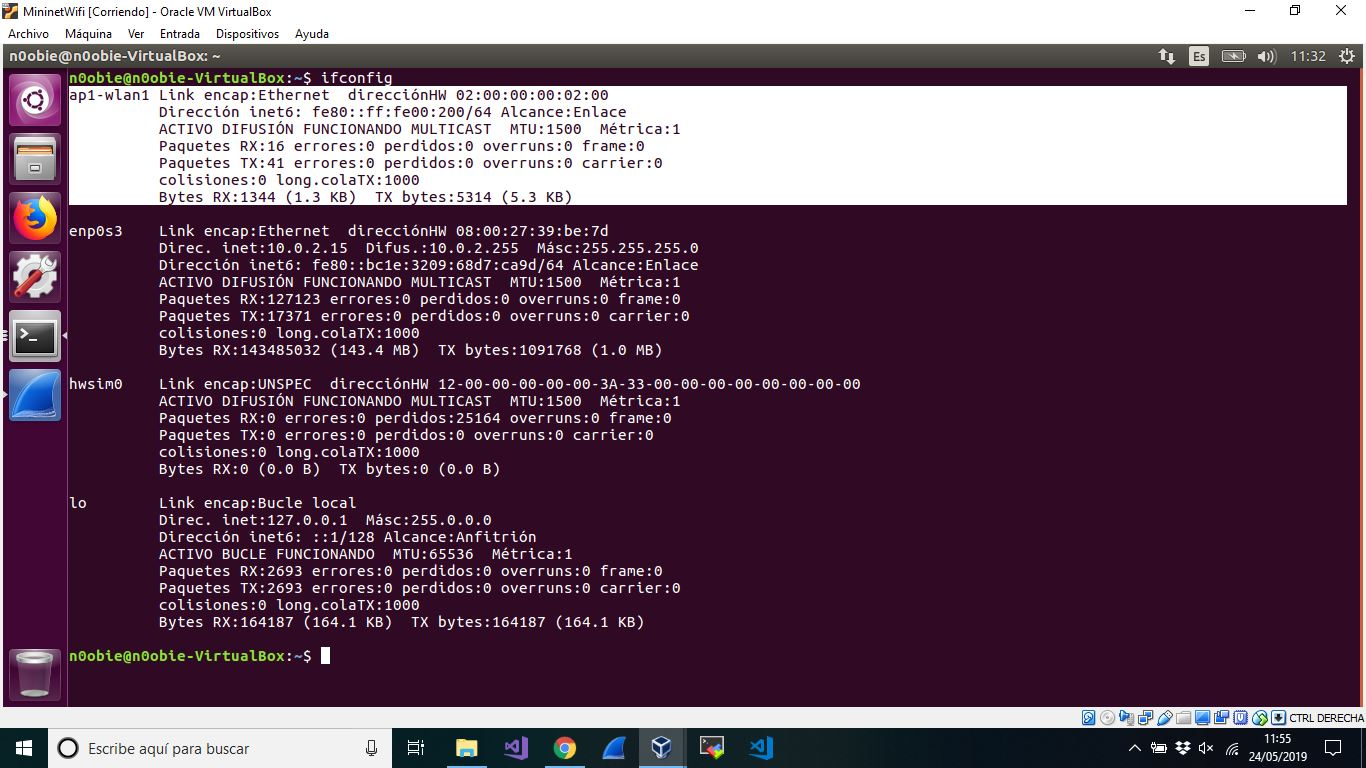
\includegraphics[width=0.9\linewidth]{./img/6.JPG}
    \caption{Interfaz ap1-wlan1 del Punto de acceso.}
  \label{fig:yo}
\end{figure}
\newpage
Si deseamos ver \textbf{paquetes OpenFlow}, debemos poner a escuchar Wireshark  en la interfaz de \textbf{loopback}. Podemos además utilizar el filtro: \textbf{OpenFlow\_1.0} para visualizarlo de una forma más clara. Dicho esto, ponemos a capturar Wireshark y repetimos el ping entre sta1 y sta2.
\begin{figure}[!htb]
  \centering
    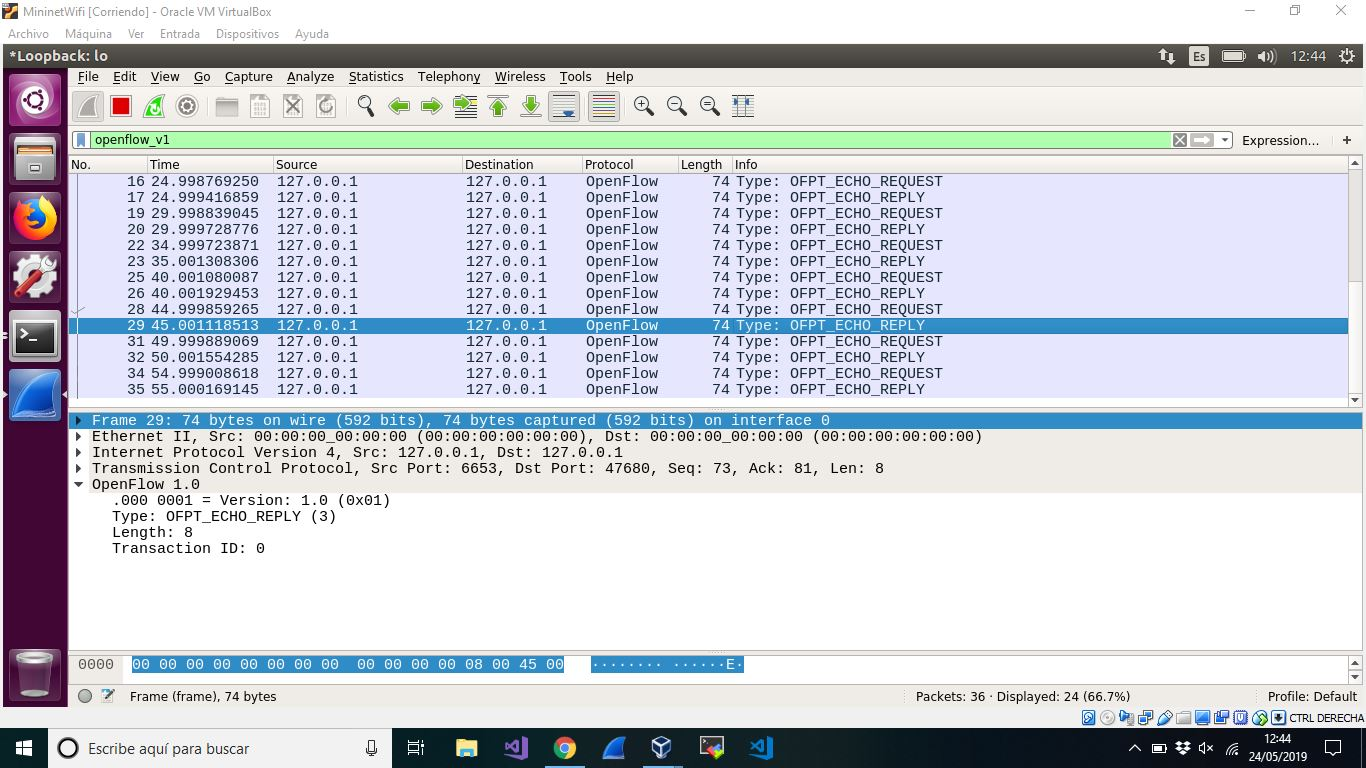
\includegraphics[width=\linewidth]{./img/7.JPG}
    \caption{Tráfico OpenFlow.}
  \label{fig:yo}
\end{figure}